\flushbottom

%% CONTINUE: This needs a lot of work.




%%=============================================================================
%%=============================================================================
\chapter{Vectors}





%%=============================================================================
\section{Vectors}


%%-----------------------------------------------------------------------------
\subsection{Scalars and Vectors}

A \textit{vector} is a quantity having both a magnitude and a direction.
Examples of vector quantities are velocity, force and position.  
One can represent a vector in $n$-dimensional space with an arrow whose
initial point is at the origin, (Figure~\ref{vector}).
The magnitude is the length of the vector.  Typographically, variables 
representing vectors are often written in capital letters, bold face or with a 
vector over-line, $A, \mathbf{a}, \vec{a}$.  The magnitude of a vector is 
denoted $| \mathbf{a} |$.

\begin{figure}[htb!]
\begin{center}
  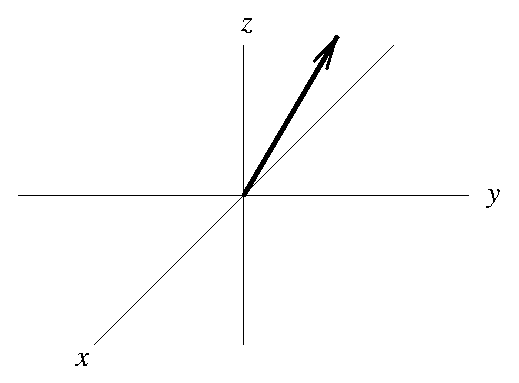
\includegraphics[width=0.4\textwidth]{algebra/vectors/vector}
\end{center}
\caption{Graphical representation of a vector in three dimensions.}
\label{vector}
\end{figure}

A \textit{scalar} has only a magnitude.  Examples of scalar quantities are
mass, time and speed.




%% CONTINUE: Introduce the concepts of a vector space.
\paragraph{Vector Algebra.}
Two vectors are equal if they have the same magnitude and direction.  
The negative of a vector, denoted $- \mathbf{a}$, is a vector of the same
magnitude as $\mathbf{a}$ but in the opposite direction.  We add two vectors
$\mathbf{a}$ and $\mathbf{b}$ by placing the tail of $\mathbf{b}$ at 
the head of $\mathbf{a}$ and defining $\mathbf{a} + \mathbf{b}$ to be 
the vector with tail at the origin and head at the head of $\mathbf{b}$.
(See Figure~\ref{addvector}.)

\begin{figure}[htb!]
\begin{center}
  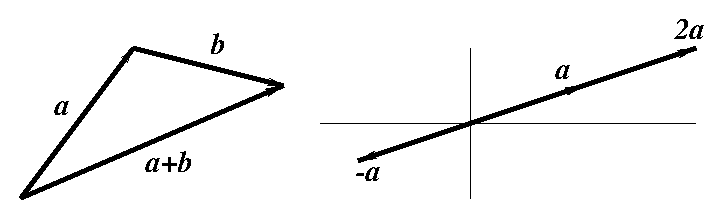
\includegraphics[width=0.5\textwidth]{algebra/vectors/addvec}
\end{center}
\caption{Vector arithmetic.}
\label{addvector}
\end{figure}

The difference, $\mathbf{a} - \mathbf{b}$, is defined as the sum of 
$\mathbf{a}$ and the negative of $\mathbf{b}$, $\mathbf{a} + (- \mathbf{b})$.
The result of multiplying $\mathbf{a}$ by a scalar $\alpha$ is a vector of 
magnitude $|\alpha|\,| \mathbf{a} |$ with the same/opposite direction if 
$\alpha$ is positive/negative.  (See Figure~\ref{addvector}.) 

Here are the properties of adding vectors and multiplying them by a 
scalar.  They are evident from geometric considerations.
\begin{alignat*}{3}
&\mathbf{a} + \mathbf{b} = \mathbf{b} + \mathbf{a} &\quad
&\alpha \mathbf{a} = \mathbf{a} \alpha &\quad
&\mathrm{commutative laws} \\
&( \mathbf{a} + \mathbf{b} ) + \mathbf{c} 
        = \mathbf{a} + ( \mathbf{b} + \mathbf{c} ) &\quad
&\alpha ( \beta \mathbf{a} ) = ( \alpha \beta ) \mathbf{a} &\quad
&\mathrm{associative laws} \\
&\alpha ( \mathbf{a} + \mathbf{b} ) 
        = \alpha \mathbf{a} + \alpha \mathbf{b} &\quad
&( \alpha + \beta ) \mathbf{a} = \alpha \mathbf{a} + \beta \mathbf{a} &\quad
&\mathrm{distributive laws}
\end{alignat*}



\paragraph{Zero and Unit Vectors.}
\index{zero vector}
\index{null vector}
The additive identity element for vectors is the \textit{zero vector} or
\textit{null vector}.  This is a vector of magnitude zero which is denoted
as $\mathbf{0}$.  A \textit{unit vector} is a vector of magnitude one.  If
$\mathbf{a}$ is nonzero then $\mathbf{a} / | \mathbf{a} |$ is a unit vector
in the direction of $\mathbf{a}$.  Unit vectors are often denoted with a caret
over-line, $\hat{\mathbf{n}}$.




\paragraph{Rectangular Unit Vectors.}
\index{rectangular unit vectors}
\index{vector!rectangular unit}
In $n$ dimensional Cartesian space, $\mathbb{R}^n$, the unit vectors in the 
directions of the coordinates axes are $\mathbf{e}_1, \ldots \mathbf{e}_n$.
These are called the \textit{rectangular unit vectors}. 
To cut down on subscripts, the unit vectors in three dimensional space 
are often denoted with $\mathbf{i}$, $\mathbf{j}$ and $\mathbf{k}$.  
(Figure~\ref{rectvec}).

\begin{figure}[htb!]
\begin{center}
  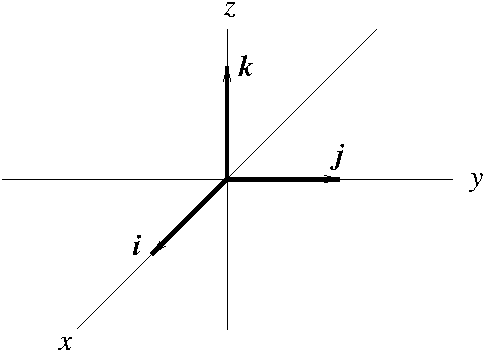
\includegraphics[width=0.4\textwidth]{algebra/vectors/rectvec}
\end{center}
\caption{Rectangular unit vectors.}
\label{rectvec}
\end{figure}



\paragraph{Components of a Vector.}
\index{vector!components of}
Consider a vector $\mathbf{a}$ with tail at the origin and head having the 
Cartesian coordinates $(a_1, \ldots, a_n)$.  We can represent this vector
as the sum of $n$ \textit{rectangular component vectors}, 
$\mathbf{a} = a_1 \mathbf{e}_1 + \cdots + a_n \mathbf{e}_n$.
(See Figure~\ref{veccomp}.)
Another notation for the vector $\mathbf{a}$ is $\langle a_1, \ldots, a_n \rangle$.
By the Pythagorean theorem, the magnitude of the vector $\mathbf{a}$ is
$| \mathbf{a} | = \sqrt{a_1^2 + \cdots + a_n^2}$.

\begin{figure}[htb!]
\begin{center}
  \includegraphics[width=0.4\textwidth]{algebra/vectors/veccomp}
\end{center}
\caption{Components of a vector.}
\label{veccomp}
\end{figure}






%%-----------------------------------------------------------------------------
\subsection{The Kronecker Delta and Einstein Summation Convention}


The Kronecker Delta tensor is defined
\[
\delta_{ij} = 
        \begin{cases}
        1 &\mathrm{if}\ i = j, \\
        0 &\mathrm{if}\ i \neq j.
        \end{cases}
\]
This notation will be useful in our work with vectors.



Consider writing a vector in terms of its rectangular components.  Instead
of using ellipses: $\mathbf{a} = a_1 \mathbf{e}_1 + \cdots + a_n \mathbf{e}_n$,
we could write the expression as a sum: 
$\mathbf{a} = \sum_{i = 1}^n a_i \mathbf{e}_i$.  We can shorten this notation
by leaving out the sum: $\mathbf{a} = a_i \mathbf{e}_i$, where it is 
understood that whenever an index is repeated in  a term we sum over that 
index from $1$ to $n$.  This is the \textit{Einstein summation convention}.
A repeated index is called a \textit{summation
index} or a \textit{dummy index}.  Other indices can take any value from $1$ to 
$n$ and are called \textit{free indices}.




\begin{Example}
Consider the matrix equation: $\mathbf{A} \cdot \mathbf{x} = \mathbf{b}$.
We can write out the matrix and vectors explicitly.
\[
\begin{pmatrix}
a_{11} & \cdots & a_{1 n} \\
\vdots & \ddots & \vdots \\
a_{n 1} & \cdots & a_{n n}
\end{pmatrix}
\begin{pmatrix}
x_1 \\
\vdots \\
x_n
\end{pmatrix}
=
\begin{pmatrix}
b_1 \\
\vdots \\
b_n
\end{pmatrix}
\]
This takes much less space when we use the summation convention.
\[
a_{i j} x_j = b_i
\]
Here $j$ is a summation index and $i$ is a free index.
\end{Example}










%%-----------------------------------------------------------------------------
\subsection{The Dot and Cross Product}


\paragraph{Dot Product.}
The \textit{dot product} or \textit{scalar product} of two vectors is
defined,
\[
\mathbf{a} \cdot \mathbf{b} \equiv | \mathbf{a} | | \mathbf{b} | \cos \theta,
\]
where $\theta$ is the angle from $\mathbf{a}$ to $\mathbf{b}$.  
From this definition one can derive the following properties:
\begin{itemize}
\item
$\mathbf{a} \cdot \mathbf{b} = \mathbf{b} \cdot \mathbf{a}$, 
commutative.
\item
$\alpha ( \mathbf{a} \cdot \mathbf{b} ) =
( \alpha \mathbf{a} ) \cdot \mathbf{b} =
\mathbf{a} \cdot ( \alpha \mathbf{b} )$, associativity of scalar 
multiplication.
\item
$\mathbf{a} \cdot ( \mathbf{b} + \mathbf{c} ) = 
\mathbf{a} \cdot \mathbf{b} + \mathbf{a} \cdot \mathbf{c}$,
distributive.  (See Exercise~\ref{exercise distributive law dot product}.)
\item
$\mathbf{e}_i \mathbf{e}_j = \delta_{i j}$.  In three dimensions, this is
\[ 
\mathbf{i} \cdot \mathbf{i} = \mathbf{j} \cdot \mathbf{j} =
\mathbf{k} \cdot \mathbf{k} = 1, \qquad
\mathbf{i} \cdot \mathbf{j} = \mathbf{j} \cdot \mathbf{k} = 
\mathbf{k} \cdot \mathbf{i} = 0. 
\]
\item
$\mathbf{a} \cdot \mathbf{b} = a_i b_i \equiv a_1 b_1 + \cdots + a_n b_n$, 
dot product in terms of rectangular components.
\item
If $\mathbf{a} \cdot \mathbf{b} = 0$ then either $\mathbf{a}$ and $\mathbf{b}$
are orthogonal, (perpendicular), or one of $\mathbf{a}$ and $\mathbf{b}$
are zero.
\end{itemize}


\paragraph{The Angle Between Two Vectors.}
We can use the dot product to find the angle between two vectors,
$\mathbf{a}$ and $\mathbf{b}$.   From the definition of the dot product,
\[
\mathbf{a} \cdot \mathbf{b} = | \mathbf{a} | | \mathbf{b} | \cos \theta.
\]
If the vectors are nonzero, then
\[
\theta = \arccos \left( \frac{ \mathbf{a} \cdot \mathbf{b} }
                { | \mathbf{a} | | \mathbf{b} | }  \right).
\]




\begin{Example}
What is the angle between $\mathbf{i}$ and $\mathbf{i} + \mathbf{j}$?
\begin{align*}
\theta
        &= \arccos \left( \frac{ \mathbf{i} \cdot (\mathbf{i} + \mathbf{j} ) }
                { | \mathbf{i} | | \mathbf{i} + \mathbf{j} | } \right) \\
        &= \arccos \left( \frac{1}{\sqrt{2}} \right) \\
        &= \frac{\pi}{4}.
\end{align*}
\end{Example}





\paragraph{Parametric Equation of a Line.}
Consider a line in $\mathbb{R}^n$ that passes through the point 
$\mathbf{a}$ and is parallel to
the vector $\mathbf{t}$, (tangent).  A parametric equation of the line is
\[
\mathbf{x} = \mathbf{a} + u \mathbf{t}, \quad u \in \mathbb{R}.
\]





\paragraph{Implicit Equation of a Line In $2D$.}
Consider a line in $\mathbb{R}^2$ that passes through the point 
$\mathbf{a}$ and is normal, (orthogonal, perpendicular), to the vector 
$\mathbf{n}$.  All the lines that are 
normal to $\mathbf{n}$ have the property that $\mathbf{x} \cdot \mathbf{n}$ is a 
constant, where $\mathbf{x}$ is any point on the line.  
(See Figure~\ref{dotlines}.)
$\mathbf{x} \cdot \mathbf{n} = 0$ is the line that is normal to $\mathbf{n}$
and passes through the origin.  The line that is normal to $\mathbf{n}$
and passes through the point $\mathbf{a}$ is
\[
\mathbf{x} \cdot \mathbf{n} = \mathbf{a} \cdot \mathbf{n}.
\]

\begin{figure}[htb!]
\begin{center}
  \includegraphics[width=0.33\textwidth]{algebra/vectors/dotlines}
\end{center}
\caption{Equation for a line.}
\label{dotlines}
\end{figure}


The normal to a line determines an orientation of the line.  The normal 
points in the direction that is above the line.  A point $\mathbf{b}$ is 
(above/on/below) the line if $(\mathbf{b} - \mathbf{a}) \cdot \mathbf{n}$ is 
(positive/zero/negative).  The signed distance of a point $\mathbf{b}$
from the line
$ \mathbf{x} \cdot \mathbf{n} = \mathbf{a} \cdot \mathbf{n}$ is 
\[
(\mathbf{b} - \mathbf{a}) \cdot \frac{\mathbf{n}}{|\mathbf{n}|}.
\]







\paragraph{Implicit Equation of a Hyperplane.}
A hyperplane in $\mathbb{R}^n$ is an $n-1$ dimensional ``sheet'' 
which passes through a given point and is normal to a given direction.
In $\mathbb{R}^3$ we call this a plane.
Consider a hyperplane that passes through the point $\mathbf{a}$ and is normal
to the vector $\mathbf{n}$.  All the hyperplanes that are normal
to $\mathbf{n}$ have the property that $\mathbf{x} \cdot \mathbf{n}$ is a constant, 
where $\mathbf{x}$ is any point in the hyperplane.  
$\mathbf{x} \cdot \mathbf{n} = 0$ is the hyperplane that is normal to $\mathbf{n}$
and passes through the origin.  The hyperplane that is normal to $\mathbf{n}$
and passes through the point $\mathbf{a}$ is
\[
\mathbf{x} \cdot \mathbf{n} = \mathbf{a} \cdot \mathbf{n}.
\]


The normal determines an orientation of the hyperplane.  The normal 
points in the direction that is above the hyperplane.  A point $\mathbf{b}$ is 
(above/on/below) the hyperplane if $(\mathbf{b} - \mathbf{a}) \cdot \mathbf{n}$ is 
(positive/zero/negative).  The signed distance of a point $\mathbf{b}$
from the hyperplane $ \mathbf{x} \cdot \mathbf{n} = \mathbf{a} \cdot \mathbf{n}$ is 
\[
(\mathbf{b} - \mathbf{a}) \cdot \frac{\mathbf{n}}{|\mathbf{n}|}.
\]







\paragraph{Right and Left-Handed Coordinate Systems.}
Consider a rectangular coordinate system in two dimensions.  Angles are 
measured from the positive $x$ axis in the direction of the positive $y$
axis.  There are two ways of labeling the axes.  (See Figure~\ref{twodimrl}.)
In one the angle increases in the counterclockwise direction and in the
other the angle increases in the clockwise direction.  The former is the 
familiar Cartesian coordinate system.

\begin{figure}[htb!]
\begin{center}
  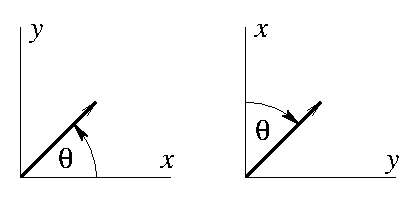
\includegraphics[width=0.3\textwidth]{algebra/vectors/twodimrl}
\end{center}
\caption{There are two ways of labeling the axes in two dimensions.}
\label{twodimrl}
\end{figure}

There are also two ways of labeling the axes in a three-dimensional
rectangular coordinate system.  These are called right-handed and 
left-handed coordinate systems.  See Figure~\ref{rlhand}. 
Any other labelling of the axes could be rotated into one of these 
configurations.  The right-handed system is the one that is used by
default.  If you put your right thumb in the 
direction of the $z$ axis in a right-handed coordinate system, then your
fingers curl in the direction from the $x$ axis to the $y$ axis.

\begin{figure}[htb!]
\begin{center}
  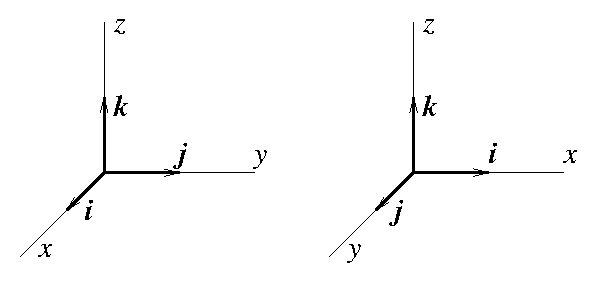
\includegraphics[width=0.4\textwidth]{algebra/vectors/rlhand}
\end{center}
\caption{Right and left handed coordinate systems.}
\label{rlhand}
\end{figure}







\paragraph{Cross Product.}
The \textit{cross product} or \textit{vector product} is defined,
\[
\mathbf{a} \times \mathbf{b} = | \mathbf{a} | | \mathbf{b} | \sin \theta \ 
\mathbf{n},
\]
where $\theta$ is the angle from $\mathbf{a}$ to $\mathbf{b}$ and 
$\mathbf{n}$ is a unit vector that is orthogonal to $\mathbf{a}$
and $\mathbf{b}$ and in the direction such that the ordered triple of
vectors $\mathbf{a}$, 
$\mathbf{b}$ and $\mathbf{n}$ form a right-handed system.

You can visualize the direction of $\mathbf{a} \times \mathbf{b}$ by applying
the \textit{right hand rule}.  Curl the fingers of your right hand in 
the direction from $\mathbf{a}$ to $\mathbf{b}$.  Your thumb points in the direction
of $\mathbf{a} \times \mathbf{b}$.  \textbf{Warning}:  Unless you are a lefty,
get in the habit of putting down your pencil before applying the right
hand rule.





The dot and cross products behave a little differently.
First note that unlike the dot product, the cross product is not 
commutative.  The magnitudes of $\mathbf{a} \times \mathbf{b}$
and $\mathbf{b} \times \mathbf{a}$ are the same, but their directions are opposite.
(See Figure~\ref{anticomm}.)

\begin{figure}[htb!]
\begin{center}
  \includegraphics[width=0.125\textwidth]{algebra/vectors/anticomm}
\end{center}
\caption{The cross product is anti-commutative.}
\label{anticomm}
\end{figure}

Let
\[
\mathbf{a} \times \mathbf{b} = | \mathbf{a} | | \mathbf{b} | \sin \theta\ \mathbf{n}
\quad \mathrm{and} \quad
\mathbf{b} \times \mathbf{a} = | \mathbf{b} | | \mathbf{a} | \sin \phi\ \mathbf{m}.
\]
The angle from $\mathbf{a}$ to $\mathbf{b}$ is the same as the angle from
$\mathbf{b}$ to $\mathbf{a}$.  Since $\{ \mathbf{a}, \mathbf{b}, \mathbf{n} \}$ and 
$\{ \mathbf{b}, \mathbf{a}, \mathbf{m} \}$ are right-handed systems, $\mathbf{m}$
points in the opposite direction as $\mathbf{n}$.  Since 
$\mathbf{a} \times \mathbf{b} = - \mathbf{b} \times \mathbf{a}$ we say that the 
cross product is anti-commutative.



Next we note that since
\[
| \mathbf{a} \times \mathbf{b} | = | \mathbf{a} | | \mathbf{b} | \sin \theta,
\]
the magnitude of $\mathbf{a} \times \mathbf{b}$ is the area of the parallelogram
defined by the two vectors.  (See Figure~\ref{paratri}.)  The area of the 
triangle defined by two vectors is then 
$\frac{1}{2} | \mathbf{a} \times \mathbf{b} |$.

\begin{figure}[htb!]
\begin{center}
  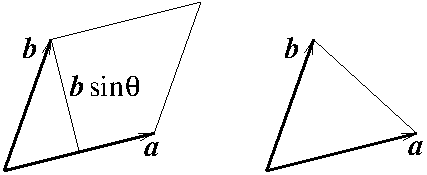
\includegraphics[width=0.33\textwidth]{algebra/vectors/paratri}
\end{center}
\caption{The parallelogram and the triangle defined by two vectors.}
\label{paratri}
\end{figure}



From the definition of the cross product, one can derive the following 
properties:
\begin{itemize}
\item
$\mathbf{a} \times \mathbf{b} = - \mathbf{b} \times \mathbf{a}$, 
anti-commutative.
\item
$\alpha ( \mathbf{a} \times \mathbf{b} ) =
( \alpha \mathbf{a} ) \times \mathbf{b} =
\mathbf{a} \times ( \alpha \mathbf{b} )$, associativity of scalar 
multiplication.
\item
$\mathbf{a} \times ( \mathbf{b} + \mathbf{c} ) = 
\mathbf{a} \times \mathbf{b} + \mathbf{a} \times \mathbf{c}$,
distributive.
\item
$( \mathbf{a} \times \mathbf{b} ) \times \mathbf{c} \neq
\mathbf{a} \times ( \mathbf{b} \times \mathbf{c} )$.  The cross 
product is not associative.
\item
$ \mathbf{i} \times \mathbf{i} = \mathbf{j} \times \mathbf{j} =
\mathbf{k} \times \mathbf{k} = 0$.
\item
$ \mathbf{i} \times \mathbf{j} = \mathbf{k}$, 
$\mathbf{j} \times \mathbf{k} = \mathbf{i}$,
$\mathbf{k} \times \mathbf{i} = \mathbf{j}$.
\item
\[
\mathbf{a} \times \mathbf{b} = 
(a_2 b_3 - a_3 b_2) \mathbf{i} + (a_3 b_1 - a_1 b_3) \mathbf{j}
+ (a_1 b_2 - a_2 b_1) \mathbf{k} =
\begin{vmatrix}
\mathbf{i} & \mathbf{j} & \mathbf{k} \\
a_1 & a_2 & a_3 \\
b_1 & b_2 & b_3
\end{vmatrix},
\]
cross product in terms of rectangular components.
\item
If $\mathbf{a} \cdot \mathbf{b} = \mathbf{0}$ then either $\mathbf{a}$ and 
$\mathbf{b}$ are parallel or one of $\mathbf{a}$ or $\mathbf{b}$ is zero.
\end{itemize}









\paragraph{Scalar Triple Product.}
Consider the volume of the parallelopiped defined by three vectors.
(See Figure~\ref{paraped}.)
The area of the base is $\left| |\mathbf{b}| |\mathbf{c}| \sin \theta \right|$, 
where $\theta$
is the angle between $\mathbf{b}$ and $\mathbf{c}$.  The height is
$| \mathbf{a} | \cos \phi$, where $\phi$ is the angle between
$\mathbf{b} \times \mathbf{c}$ and $\mathbf{a}$.  Thus the volume of 
the parallelopiped is 
$|\mathbf{a}| |\mathbf{b}| |\mathbf{c}| \sin \theta \cos \phi$.

\begin{figure}[htb!]
\begin{center}
  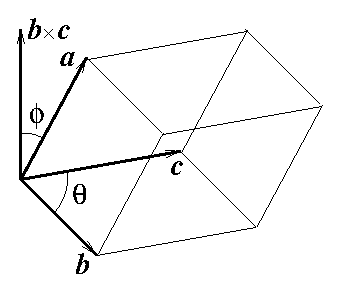
\includegraphics[width=0.25\textwidth]{algebra/vectors/paraped}
\end{center}
\caption{The parallelopiped defined by three vectors.}
\label{paraped}
\end{figure}

Note that 
\begin{align*}
\left| \mathbf{a} \cdot (\mathbf{b} \times \mathbf{c}) \right|
        &= \left| \mathbf{a} \cdot ( |\mathbf{b}| |\mathbf{c}| \sin \theta \ \mathbf{n} ) 
                \right| \\
        &= \left| |\mathbf{a}| |\mathbf{b}| |\mathbf{c}| \sin \theta \cos \phi \right|.
\end{align*}
Thus $\left| \mathbf{a} \cdot (\mathbf{b} \times \mathbf{c}) \right|$ is the volume of 
the parallelopiped.  $\mathbf{a} \cdot ( \mathbf{b} \times \mathbf{c} )$ is the volume
or the negative of the volume depending on whether 
$\{\mathbf{a}, \mathbf{b},\mathbf{c}\}$ is a right or left-handed system.

Note that parentheses are unnecessary in 
$\mathbf{a} \cdot \mathbf{b} \times \mathbf{c}$.  There is only one way to 
interpret the expression.  If you did the dot product first then you
would be left with the cross product of a scalar and a vector 
which is meaningless.  $\mathbf{a} \cdot \mathbf{b} \times \mathbf{c}$ is called
the \textit{scalar triple product}.


\paragraph{Plane Defined by Three Points.}
Three points which are not collinear define a plane.  Consider a plane 
that passes through the three points $\mathbf{a}$, $\mathbf{b}$ and $\mathbf{c}$.
One way of expressing that the point $\mathbf{x}$ lies in the plane is that 
the vectors $\mathbf{x} - \mathbf{a}$, $\mathbf{b} - \mathbf{a}$ and $\mathbf{c} - \mathbf{a}$ 
are coplanar.  (See Figure~\ref{stpplane}.)
If the vectors are coplanar, then the parallelopiped
defined by these three vectors will have zero volume.  We can express this
in an equation using the scalar triple product,
\[
(\mathbf{x} - \mathbf{a}) \cdot (\mathbf{b} - \mathbf{a}) \times (\mathbf{c} - \mathbf{a}) = 0.
\]

\begin{figure}[htb!]
\begin{center}
  \includegraphics[width=0.2\textwidth]{algebra/vectors/stpplane}
\end{center}
\caption{Three points define a plane.}
\label{stpplane}
\end{figure}







%% CONTINUE: Edit this to fit in this chapter.
%%============================================================================
\section{Sets of Vectors in n Dimensions}

\paragraph{Orthogonality.}
Consider two $n$-dimensional vectors
\[
\mathbf{x} = (x_1, x_2, \ldots, x_n), \qquad
        \mathbf{y} = (y_1, y_2, \ldots, y_n).
\]
The inner product of these vectors can be defined
\[
\langle \mathbf{x} | \mathbf{y} \rangle \equiv
\mathbf{x} \cdot \mathbf{y} = \sum_{i=1}^n x_i y_i.
\]
The vectors are orthogonal if $\mathbf{x} \cdot \mathbf{y} = 0$.  The norm of
a vector is the length of the vector generalized to $n$ dimensions.
\[
\| \mathbf{x} \| = \sqrt{\mathbf{x} \cdot \mathbf{x}}
\]

Consider a set of vectors
\[ \{\mathbf{x}_1, \mathbf{x}_2, \ldots, \mathbf{x}_m\}.\]
If each pair of vectors in the set is orthogonal, then the set is orthogonal.
\[
\mathbf{x}_i \cdot \mathbf{x}_j = 0 \quad \mathrm{if}\ i \neq j
\]
If in addition each vector in the set has norm $1$, then the set is
orthonormal.
\[
\mathbf{x}_i \cdot \mathbf{x}_j = \delta_{i j} =
        \begin{cases}
        1 \quad &\mathrm{if}\ i = j \\
        0 \quad &\mathrm{if}\ i \neq j
        \end{cases}
\]
Here $\delta_{i j}$ is known as the Kronecker delta function.
\index{Kronecker delta function}
\index{delta function!Kronecker}


\paragraph{Completeness.}
\index{completeness!sets of vectors}
A set of $n$, $n$-dimensional vectors
\[
\{\mathbf{x}_1, \mathbf{x}_2, \ldots, \mathbf{x}_n\}
\]
is \textit{complete} if any $n$-dimensional
vector can be written as a linear combination of the vectors in the set.
That is, any vector $\mathbf{y}$ can be written
\[
\mathbf{y} = \sum_{i=1}^n c_i \mathbf{x}_i.
\]
Taking the inner product of each side of this equation with $\mathbf{x}_m$,
\begin{align*}
\mathbf{y} \cdot \mathbf{x}_m &= \left( \sum_{i=1}^n c_i \mathbf{x}_i \right)
        \cdot \mathbf{x}_m \\
        &= \sum_{i=1}^n c_i \mathbf{x}_i \cdot \mathbf{x}_m \\
        &= c_m \mathbf{x}_m \cdot \mathbf{x}_m \\
c_m     &= \frac{\mathbf{y} \cdot \mathbf{x}_m }{\| \mathbf{x}_m \|^2}
\end{align*}
Thus $\mathbf{y}$ has the expansion
\[
\mathbf{y} = \sum_{i=1}^n \frac{\mathbf{y} \cdot \mathbf{x}_i }{\| \mathbf{x}_i \|^2} \mathbf{x}_i.
\]
If in addition the set is orthonormal, then
\[
\mathbf{y} = \sum_{i=1}^n (\mathbf{y} \cdot \mathbf{x}_i) \mathbf{x}_i.
\]














\raggedbottom
%%=============================================================================
\exercises{
\pagebreak
\flushbottom
\section{Exercises}


%% CONTINUE
%% A paraboloid collects plane waves.


%%-----------------------------------------------------------------------------
\begin{large}
\noindent
\textbf{The Dot and Cross Product}
\end{large}



%% Prove the distributive law for the dot product,
\begin{Exercise}
\label{exercise distributive law dot product}
Prove the distributive law for the dot product,
\[
\mathbf{a} \cdot ( \mathbf{b} + \mathbf{c} ) 
= \mathbf{a} \cdot \mathbf{b} + \mathbf{a} \cdot \mathbf{c}.
\]

\hintsolution{distributive law dot product}
\end{Exercise}



%% \mathbf{a} \cdot \mathbf{b} = a_1 b_1 + a_2 b_2 + a_3 b_3.
\begin{Exercise}
\label{exercise a.b = ai bi}
Prove that
\[
\mathbf{a} \cdot \mathbf{b} = a_i b_i \equiv a_1 b_1 + \cdots + a_n b_n.
\]

\hintsolution{a.b = ai bi}
\end{Exercise}




%% What is the angle?
\begin{Exercise}
\label{exercise angle between i+j i+3j}
What is the angle between the vectors $\mathbf{i} + \mathbf{j}$ and
$\mathbf{i} + 3 \mathbf{j}$?

\hintsolution{angle between i+j i+3j}
\end{Exercise}




%% Prove the distributive law for the cross product,
\begin{Exercise}
\label{exercise distributive law cross product}
Prove the distributive law for the cross product,
\[
\mathbf{a} \times ( \mathbf{b} + \mathbf{c} ) 
= \mathbf{a} \times \mathbf{b} + \mathbf{a} \times \mathbf{b}.
\]

\hintsolution{distributive law cross product}
\end{Exercise}



%% Matrix form of cross product
\begin{Exercise}
\label{exercise matrix form of cross product}
Show that
\[
\mathbf{a} \times \mathbf{b} =
\begin{vmatrix}
\mathbf{i} & \mathbf{j} & \mathbf{k} \\
a_1 & a_2 & a_3 \\
b_1 & b_2 & b_3
\end{vmatrix}
\]

\hintsolution{matrix form of cross product}
\end{Exercise}




%% What is the area of the quadrilateral?
\begin{Exercise}
\label{exercise area quadrilateral 11 42 37 23}
What is the area of the quadrilateral with vertices at $(1,1)$, $(4,2)$,
$(3,7)$ and $(2,3)$?

\hintsolution{area quadrilateral 11 42 37 23}
\end{Exercise}



%% What is the volume of the tetrahedron?
\begin{Exercise}
\label{exercise volume tetrahedron 110 321 241 125}
What is the volume of the tetrahedron with vertices at $(1,1,0)$, $(3,2,1)$,
$(2,4,1)$ and $(1,2,5)$?

\hintsolution{volume tetrahedron 110 321 241 125}
\end{Exercise}




%% What is the equation of the plane that passes through the points
\begin{Exercise}
\label{exercise equation of plane 123 231 312}
What is the equation of the plane that passes through the points
$(1,2,3)$, $(2,3,1)$ and $(3,1,2)$?  What is the distance from the point
$(2,3,5)$ to the plane?

\hintsolution{equation of plane 123 231 312}
\end{Exercise}













\raggedbottom
}
%%=============================================================================
\hints{
\pagebreak
\flushbottom
\section{Hints}




%%-----------------------------------------------------------------------------
\begin{large}
\noindent
\textbf{The Dot and Cross Product}
\end{large}




%% Prove the distributive law for the dot product,
\begin{Hint}
\label{hint distributive law dot product}
First prove the distributive law when the first vector is of unit length,
\[
\mathbf{n} \cdot ( \mathbf{b} + \mathbf{c} ) 
= \mathbf{n} \cdot \mathbf{b} + \mathbf{n} \cdot \mathbf{c}.
\]
Then all the quantities in the equation are projections onto the unit vector
$\mathbf{n}$ and you can use geometry.
\end{Hint}




%% \mathbf{a} \cdot \mathbf{b} = a_1 b_1 + a_2 b_2 + a_3 b_3.
\begin{Hint}
\label{hint a.b = ai bi}
First prove that the dot product of a rectangular unit vector with itself
is one and the dot product of two distinct rectangular unit vectors is 
zero.  Then write $\mathbf{a}$ and $\mathbf{b}$ in rectangular components 
and use the distributive law.
\end{Hint}



%% What is the angle?
\begin{Hint}
\label{hint angle between i+j i+3j}
Use $\mathbf{a} \cdot \mathbf{b} = | \mathbf{a} | | \mathbf{b} | \cos \theta$.
\end{Hint}




%% Prove the distributive law for the cross product,
\begin{Hint}
\label{hint distributive law cross product}
First consider the case that both $\mathbf{b}$ and $\mathbf{c}$ are orthogonal to 
$\mathbf{a}$.  Prove the distributive law in this case from geometric 
considerations.

Next consider two arbitrary vectors $\mathbf{a}$ and $\mathbf{b}$.  We can write 
$\mathbf{b} = \mathbf{b}_\perp + \mathbf{b}_\parallel$ where $\mathbf{b}_\perp$ is 
orthogonal to $\mathbf{a}$ and $\mathbf{b}_\parallel$ is parallel to $\mathbf{a}$.
Show that
\[
\mathbf{a} \times \mathbf{b} = \mathbf{a} \times \mathbf{b}_\perp.
\]

Finally prove the distributive law for arbitrary $\mathbf{b}$ and $\mathbf{c}$.
\end{Hint}







%% Matrix form of cross product
\begin{Hint}
\label{hint matrix form of cross product}
Write the vectors in their rectangular components and use,
\[
\mathbf{i} \times \mathbf{j} = \mathbf{k}, \quad
\mathbf{j} \times \mathbf{k} = \mathbf{i}, \quad
\mathbf{k} \times \mathbf{i} = \mathbf{j},
\]
and, 
\[
\mathbf{i} \times \mathbf{i} = 
\mathbf{j} \times \mathbf{j} = 
\mathbf{k} \times \mathbf{k} = 0.
\]
\end{Hint}



%% What is the area of the quadrilateral?
\begin{Hint}
\label{hint area quadrilateral 11 42 37 23}
The quadrilateral is composed of two triangles.
The area of a triangle defined by the two vectors $\mathbf{a}$ and 
$\mathbf{b}$ is $\frac{1}{2} | \mathbf{a} \cdot \mathbf{b} |$.
\end{Hint}





%% What is the volume of the tetrahedron?
\begin{Hint}
\label{hint volume tetrahedron 110 321 241 125}
Justify that the area of a tetrahedron determined by three vectors is one 
sixth the area of the parallelogram determined by those three vectors.
The area of a parallelogram determined by three vectors is the magnitude of
the scalar triple product of the vectors: 
$\mathbf{a} \cdot \mathbf{b} \times \mathbf{c}$.
\end{Hint}







%% What is the equation of the plane that passes through the points
\begin{Hint}
\label{hint equation of plane 123 231 312}
The equation of a line that is orthogonal to $\mathbf{a}$ and passes
through the point $\mathbf{b}$ is $\mathbf{a} \cdot \mathbf{x} = 
\mathbf{a} \cdot \mathbf{b}$.  The distance of a point $\mathbf{c}$ 
from the plane is 
\[
\left | (\mathbf{c} - \mathbf{b} ) \cdot \frac{ \mathbf{a} }
{ | \mathbf{a} | } \right|
\]
\end{Hint}





\raggedbottom
}
%%=============================================================================
\solutions{
\pagebreak
\flushbottom
\section{Solutions}


%%-----------------------------------------------------------------------------
\begin{large}
\noindent
\textbf{The Dot and Cross Product}
\end{large}



%% Prove the distributive law for the dot product,
\begin{Solution}
\label{solution distributive law dot product}
First we prove the distributive law when the first vector is of unit length, 
i.e.,
\begin{equation}
\label{dotdistnorm}
\mathbf{n} \cdot ( \mathbf{b} + \mathbf{c} ) 
= \mathbf{n} \cdot \mathbf{b} + \mathbf{n} \cdot \mathbf{c}.
\end{equation}
From Figure~\ref{dotdist} we see that the projection of the vector 
$\mathbf{b} + \mathbf{c}$ onto $\mathbf{n}$ 
is equal to the sum of the projections 
$\mathbf{b} \cdot \mathbf{n}$ and $\mathbf{c} \cdot \mathbf{n}$.  

\begin{figure}[htb!]
\begin{center}
  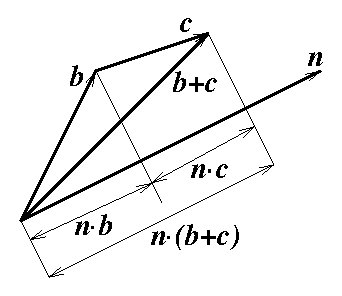
\includegraphics[width=0.3\textwidth]{algebra/vectors/dotdist}
\end{center}
\caption{The distributive law for the dot product.}
\label{dotdist}
\end{figure}

Now we extend the result to the case when the first vector has arbitrary
length.  We define $\mathbf{a} = | \mathbf{a} | \mathbf{n}$ and multiply
Equation~\ref{dotdistnorm} by the scalar, $| \mathbf{a} |$.
\begin{gather*}
| \mathbf{a} | \mathbf{n} \cdot ( \mathbf{b} + \mathbf{c} ) 
  = | \mathbf{a} | \mathbf{n} \cdot \mathbf{b} 
  + | \mathbf{a} | \mathbf{n} \cdot \mathbf{c} \\
\boxed{
\mathbf{a} \cdot ( \mathbf{b} + \mathbf{c} ) 
  = \mathbf{a} \cdot \mathbf{b} + \mathbf{a} \cdot \mathbf{c}.
}
\end{gather*}
\end{Solution}







%% \mathbf{a} \cdot \mathbf{b} = a_1 b_1 + a_2 b_2 + a_3 b_3.
\begin{Solution}
\label{solution a.b = ai bi}
First note that
\[
\mathbf{e}_i \cdot \mathbf{e}_i = | \mathbf{e}_i || \mathbf{e}_i | \cos(0) = 1.
\]
Then note that that dot product of any two distinct rectangular 
unit vectors is zero because they are orthogonal.
Now we write $\mathbf{a}$ and $\mathbf{b}$ in terms of their rectangular
components and use the distributive law.
\begin{align*}
\mathbf{a} \cdot \mathbf{b}
        &= a_i \mathbf{e}_i \cdot b_j \mathbf{e}_j \\
        &= a_i b_j \mathbf{e}_i \cdot \mathbf{e}_j \\
        &= a_i b_j \delta_{i j} \\
        &= a_i b_i
\end{align*}
\end{Solution}





%% What is the angle?
\begin{Solution}
\label{solution angle between i+j i+3j}
Since $\mathbf{a} \cdot \mathbf{b} = | \mathbf{a} | | \mathbf{b} |
\cos \theta$, we have
\[
\theta = \arccos \left( \frac{\mathbf{a} \cdot \mathbf{b}}
        {| \mathbf{a} | | \mathbf{b} | } \right)
\]
when $\mathbf{a}$ and $\mathbf{b}$ are nonzero.
\[
\theta = \arccos \left( \frac
        { (\mathbf{i} + \mathbf{j} ) \cdot ( \mathbf{i} + 3 \mathbf{j} ) }
        { |\mathbf{i} + \mathbf{j} | | \mathbf{i} + 3 \mathbf{j} | } \right)
= \arccos \left( \frac{4}{\sqrt{2} \sqrt{10}} \right)
= \arccos \left( \frac{2 \sqrt{5}}{5} \right)
\approx 0.463648
\]
\end{Solution}





%% Prove the distributive law for the cross product,
\begin{Solution}
\label{solution distributive law cross product}
First consider the case that both $\mathbf{b}$ and $\mathbf{c}$ are orthogonal to 
$\mathbf{a}$.  $\mathbf{b} + \mathbf{c}$ is the diagonal of the parallelogram
defined by $\mathbf{b}$ and $\mathbf{c}$, (see Figure~\ref{crossdst}).
Since $\mathbf{a}$ is orthogonal to each of these vectors, taking the cross
product of $\mathbf{a}$ with these vectors has the effect of rotating the
vectors through $\pi/2$ radians about $\mathbf{a}$ and multiplying their 
length by $|\mathbf{a}|$.   Note that $\mathbf{a} \times (\mathbf{b} + \mathbf{c})$
is the diagonal of the parallelogram defined by $\mathbf{a} \times \mathbf{b}$
and $\mathbf{a} \times \mathbf{c}$.  Thus we see that the distributive law holds
when $\mathbf{a}$ is orthogonal to both $\mathbf{b}$ and $\mathbf{c}$,
\[
\mathbf{a} \times ( \mathbf{b} + \mathbf{c} ) 
= \mathbf{a} \times \mathbf{b} + \mathbf{a} \times \mathbf{c}.
\]

\begin{figure}[htb!]
\begin{center}
  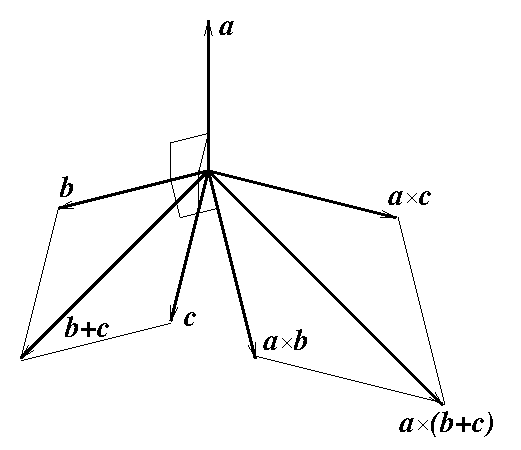
\includegraphics[width=0.4\textwidth]{algebra/vectors/crossdst}
\end{center}
\caption{The distributive law for the cross product.}
\label{crossdst}
\end{figure}

Now consider two arbitrary vectors $\mathbf{a}$ and $\mathbf{b}$.  We can write 
$\mathbf{b} = \mathbf{b}_\perp + \mathbf{b}_\parallel$ where $\mathbf{b}_\perp$ is 
orthogonal to $\mathbf{a}$ and $\mathbf{b}_\parallel$ is parallel to $\mathbf{a}$,
(see Figure~\ref{vperppar}).  

\begin{figure}[htb!]
\begin{center}
  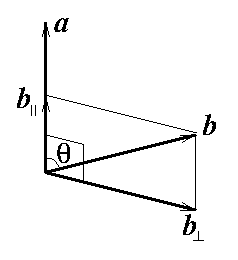
\includegraphics[width=0.2\textwidth]{algebra/vectors/vperppar}
\end{center}
\caption{The vector \textbf{b} written as a sum of components orthogonal
  and parallel to \textbf{a}.}
\label{vperppar}
\end{figure}

By the definition of the cross product,
\[
\mathbf{a} \times \mathbf{b} = | \mathbf{a} | | \mathbf{b} | \sin \theta \ \mathbf{n}.
\]
Note that 
\[
| \mathbf{b}_\perp | = | \mathbf{b} | \sin \theta,
\]
and that $\mathbf{a} \times \mathbf{b}_\perp$ is a vector in the same direction
as $\mathbf{a} \times \mathbf{b}$.  Thus we see that
\begin{align*}
\mathbf{a} \times \mathbf{b} 
        &= | \mathbf{a} | | \mathbf{b} | \sin \theta \ \mathbf{n} \\
        &= | \mathbf{a} | ( \sin \theta  | \mathbf{b} | ) \mathbf{n} \\
        &= | \mathbf{a} | | \mathbf{b}_\perp | \mathbf{n} 
        &= | \mathbf{a} | | \mathbf{b}_\perp | \sin(\pi/2) \mathbf{n} 
\end{align*}
\[
\mathbf{a} \times \mathbf{b} = \mathbf{a} \times \mathbf{b}_\perp.
\]

Now we are prepared to prove the distributive law for arbitrary $\mathbf{b}$
and $\mathbf{c}$.
\begin{align*}
\mathbf{a} \times ( \mathbf{b} + \mathbf{c} )
        &= \mathbf{a} \times ( \mathbf{b}_\perp + \mathbf{b}_\parallel 
                + \mathbf{c}_\perp + \mathbf{c}_\parallel ) \\
        &= \mathbf{a} \times ( ( \mathbf{b} + \mathbf{c} )_\perp 
                + ( \mathbf{b} + \mathbf{c} )_\parallel ) \\
        &= \mathbf{a} \times ( ( \mathbf{b} + \mathbf{c} )_\perp ) \\
        &= \mathbf{a} \times \mathbf{b}_\perp + \mathbf{a} \times \mathbf{c}_\perp \\
        &= \mathbf{a} \times \mathbf{b}+ \mathbf{a} \times \mathbf{c}
\end{align*}
\[
\boxed{
\mathbf{a} \times ( \mathbf{b} + \mathbf{c} )
        = \mathbf{a} \times \mathbf{b}+ \mathbf{a} \times \mathbf{c}
}
\]
\end{Solution}




%% Matrix form of cross product
\begin{Solution}
\label{solution matrix form of cross product}
We know that 
\[
\mathbf{i} \times \mathbf{j} = \mathbf{k}, \quad
\mathbf{j} \times \mathbf{k} = \mathbf{i}, \quad
\mathbf{k} \times \mathbf{i} = \mathbf{j},
\]
and that
\[
\mathbf{i} \times \mathbf{i} = 
\mathbf{j} \times \mathbf{j} = 
\mathbf{k} \times \mathbf{k} = 0.
\]
Now we write $\mathbf{a}$ and $\mathbf{b}$ in terms of their rectangular
components and use the distributive law to expand the cross product.
\begin{align*}
\mathbf{a} \times \mathbf{b}
        &= (a_1 \mathbf{i} + a_2 \mathbf{j} + a_3 \mathbf{k} ) \times
          (b_1 \mathbf{i} + b_2 \mathbf{j} + b_3 \mathbf{k} ) \\
        &= a_1 \mathbf{i} \times
          (b_1 \mathbf{i} + b_2 \mathbf{j} + b_3 \mathbf{k} ) 
        + a_2 \mathbf{j} \times
          (b_1 \mathbf{i} + b_2 \mathbf{j} + b_3 \mathbf{k} ) 
        + a_3 \mathbf{k} \times
          (b_1 \mathbf{i} + b_2 \mathbf{j} + b_3 \mathbf{k} ) \\
        &= a_1 b_2 \mathbf{k} + a_1 b_3 (- \mathbf{j})
        + a_2 b_1 (- \mathbf{k}) + a_2 b_3 \mathbf{i}
        + a_3 b_1 \mathbf{j} + a_3 b_2 (- \mathbf{i}) \\
        &= (a_2 b_3 - a_3 b_2) \mathbf{i} - (a_1 b_3 - a_3 b_1) \mathbf{j}
        + (a_1 b_2 - a_2 b_1) \mathbf{k}
\end{align*}
Next we evaluate the determinant.
\begin{align*}
\begin{vmatrix}
\mathbf{i} & \mathbf{j} & \mathbf{k} \\
a_1 & a_2 & a_3 \\
b_1 & b_2 & b_3
\end{vmatrix}
        &=      \mathbf{i}
                \begin{vmatrix}
                a_2 & a_3 \\
                b_2 & b_3 
                \end{vmatrix}
                - \mathbf{j}
                \begin{vmatrix}
                a_1 & a_3 \\
                b_1 & b_3 
                \end{vmatrix}
                + \mathbf{k}
                \begin{vmatrix}
                a_1 & a_2 \\
                b_1 & b_2 
                \end{vmatrix} \\
        &= (a_2 b_3 - a_3 b_2) \mathbf{i} - (a_1 b_3 - a_3 b_1) \mathbf{j}
        + (a_1 b_2 - a_2 b_1) \mathbf{k}
\end{align*}
Thus we see that,
\[
\mathbf{a} \times \mathbf{b} =
\begin{vmatrix}
\mathbf{i} & \mathbf{j} & \mathbf{k} \\
a_1 & a_2 & a_3 \\
b_1 & b_2 & b_3
\end{vmatrix}
\]
\end{Solution}




%% What is the area of the quadrilateral?
\begin{Solution}
\label{solution area quadrilateral 11 42 37 23}
The area area of the quadrilateral is the area of two triangles.  The first
triangle is defined by the vector from $(1,1)$ to $(4,2)$ and the vector
from $(1,1)$ to $(2,3)$.  The second triangle is defined by the vector from
$(3,7)$ to $(4,2)$ and the vector from $(3,7)$ to $(2,3)$. 
(See Figure~\ref{quad}.)
The area of a triangle defined by the two vectors $\mathbf{a}$ and 
$\mathbf{b}$ is $\frac{1}{2} | \mathbf{a} \cdot \mathbf{b} |$.
The area of the quadrilateral is then,
\[
\frac{1}{2} |(3 \mathbf{i} + \mathbf{j} ) \cdot ( \mathbf{i} + 2 \mathbf{j} )|
+ \frac{1}{2} |(\mathbf{i} - 5 \mathbf{j}) \cdot (-\mathbf{i} - 4 \mathbf{j} )|
= \frac{1}{2} (5) + \frac{1}{2} (19)
= 12.
\]

\begin{figure}[htb!]
\begin{center}
  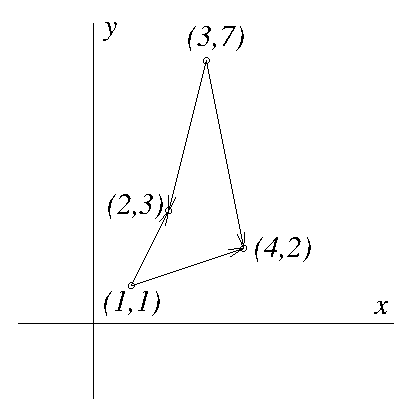
\includegraphics[width=0.3\textwidth]{algebra/vectors/quad}
\end{center}
\caption{Quadrilateral.}
\label{quad}
\end{figure}
\end{Solution}



%% What is the volume of the tetrahedron?
\begin{Solution}
\label{solution volume tetrahedron 110 321 241 125}
The tetrahedron is determined by the three vectors with tail at $(1,1,0)$
and heads at $(3,2,1)$, $(2,4,1)$ and $(1,2,5)$.  These are
$\langle 2,1,1 \rangle$, $\langle 1,3,1 \rangle$ and $\langle 0,1,5 \rangle$.  The area of the
tetrahedron is one sixth the area of the parallelogram determined by
these vectors.  (This is because the area of a pyramid is 
$\frac{1}{3} (\mathrm{base})(\mathrm{height})$.  The base of the tetrahedron is
half the area of the parallelogram and the heights are the same.
$\frac{1}{2} \frac{1}{3} = \frac{1}{6}$ )
Thus the area of a tetrahedron determined by three
vectors is $\frac{1}{6} | \mathbf{a} \cdot \mathbf{b} \times \mathbf{c} |$.
The area of the tetrahedron is
\[
\frac{1}{6} \left| \langle 2,1,1 \rangle \cdot \langle 1,3,1 \rangle \times \langle 1,2,5 \rangle 
        \right|
= \frac{1}{6} \left| \langle 2,1,1 \rangle \cdot \langle 13,-4,-1 \rangle \right|
= \frac{7}{2} 
\]
\end{Solution}


%% What is the equation of the plane that passes through the points
\begin{Solution}
\label{solution equation of plane 123 231 312}
The two vectors with tails at $(1,2,3)$ and heads at $(2,3,1)$ and $(3,1,2)$
are parallel to the plane.  Taking the cross product of these two vectors
gives us a vector that is orthogonal to the plane.
\[
\langle 1,1,-2 \rangle \times \langle 2,-1,-1 \rangle = \langle -3,-3,-3 \rangle
\]
We see that the plane is orthogonal to the vector $\langle 1,1,1 \rangle$ and passes
through the point $(1,2,3)$.  The equation of the plane is
\[
\langle 1,1,1 \rangle \cdot \langle x,y,z \rangle = \langle 1,1,1 \rangle \cdot \langle 1,2,3 \rangle,
\]
\[
x + y + z = 6.
\]
Consider the vector with tail at $(1,2,3)$ and head at $(2,3,5)$.  The
magnitude of the dot product of this vector with the unit normal vector gives
the distance from the plane.
\[
\left| \langle 1,1,2 \rangle \cdot \frac{ \langle 1,1,1 \rangle }{ | \langle 1,1,1 \rangle | } \right|
= \frac{4}{\sqrt{3}}
= \frac{4 \sqrt{3}}{3}
\]
\end{Solution}







\raggedbottom
}
